% Created 2019-11-12 Tue 16:10
% Intended LaTeX compiler: pdflatex
\documentclass{article}
\usepackage[utf8]{inputenc}
\usepackage[T1]{fontenc}
\usepackage{graphicx}
\usepackage{grffile}
\usepackage{longtable}
\usepackage{wrapfig}
\usepackage{rotating}
\usepackage[normalem]{ulem}
\usepackage{amsmath}
\usepackage{textcomp}
\usepackage{amssymb}
\usepackage{capt-of}
\usepackage{hyperref}
\bibliographystyle{plain}
\author{Britt Anderson}
\date{\today}
\title{testRBabel}
\hypersetup{
 pdfauthor={Britt Anderson},
 pdftitle={testRBabel},
 pdfkeywords={},
 pdfsubject={},
 pdfcreator={Emacs 26.3 (Org mode 9.2.6)}, 
 pdflang={English}}
\begin{document}

\maketitle
\tableofcontents

This is to test your installation of the files and programs needed to make a simple report. To compile to pdf use \texttt{C-c C-e l p}.

This loads an R library
\begin{verbatim}
library(random)
\end{verbatim}


Now we will see if we can some source code and a simple plot for our export.

\begin{verbatim}
x = 1:10
y = rnorm(10)
print(mean(y))
\end{verbatim}

\begin{verbatim}
plot(x,y,type = 'b')
\end{verbatim}

\begin{center}
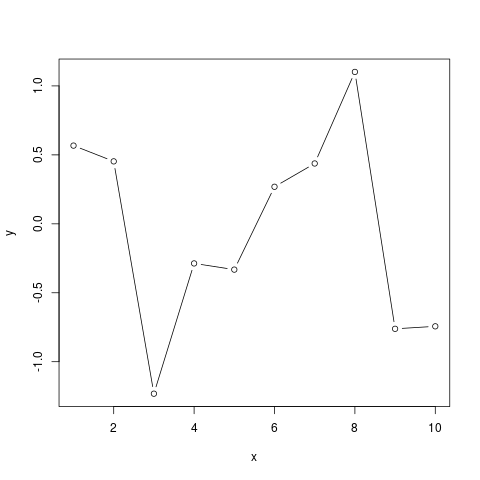
\includegraphics[width=.9\linewidth]{simplePlot.png}
\end{center}

\section{Testing Citations}
\label{sec:orge7ea477}
\end{document}

This stackexchange \href{https://tex.stackexchange.com/questions/114864/how-to-get-bibtex-to-work-with-org-mode-latex-export}{question} may be useful if you have trouble getting things to work. 

And the ta in the class wrote this article \cite{turpin2019bullshit}


\end{document}

I wrote a book about using computers in psychology \cite{anderson2014computational}.




\bibliography{mytest}
\end{document}
